% !TEX root = ../main.tex
\chapter{はじめに}

\section{一つの送信}

昼休み、利用者がブラウザで社内のAIアプリを開きます。入力欄へ「注文番号1234はいつ届きますか」と打ち込み、送信ボタンを押します。少し待つと、「明日の午後に到着する予定です」という応答が画面へ現れます。利用者から見れば、起きたことはこれだけです。

しかし、送信から応答までの数秒には、広い範囲の技術が折り重なっています。指やキーボードの操作は、電気の状態の変化である\term{電気信号}へ変わります。その信号を受け取る\term{CPU}は「中央処理装置」を意味し、計算と機械全体の制御を進める部品です。CPUは、何を計算するかを細かく指示した\term{命令}を一つずつ実行します。

動いているプログラムと機械の間には、\term{OS}があります。OSは「オペレーティングシステム」の略で、機械の動きを管理するプログラムです。複数のプログラムへCPUを使う時間、値を置く\term{メモリ}、通信する手段を安全に分けます。アプリのプログラムはOSからこれらを借り、入力を処理できる形のデータへ組み直します。

要求は、第三者に内容を読まれにくい形へ変える\term{暗号化}を受け、機器同士を結ぶ通信網である\term{ネットワーク}を渡ります。要求を受けて処理を提供する側のコンピュータを\term{サーバー}と呼びます。サーバー上のアプリケーションは注文情報を読み出し、その情報を\term{言語モデル}へ渡します。言語モデルは、文中で次に続きやすい言葉を数値計算によって選ぶ仕組みです。こうして作られた応答が、来た道を逆向きに戻ります。

本書は、この一回の送信を途中で止め、見えない仕組みを下から順にたどる物語です。最初に電気を動かそうとする力の差である電圧まで降り、そこから0と1を扱う論理回路、CPU、プログラミング言語、OS、データ、設計、ネットワーク、機械学習へ上がります。\term{機械学習}とは、処理の規則をすべて人が書く代わりに、例となるデータから規則を調整する方法です。最後に同じ画面へ戻ったとき、短い応答の背後にある因果関係を、自分の言葉で説明できることを目指します。

\begin{chapterabstract}
主役は特定の製品やプログラミング言語ではなく、一つの要求を次の層へ渡していくデータです。各層は受け取った表現を読み、仕事をし、次の表現へ変えて渡します。その境界で何が保証され、何が失われるかを追うと、離れて見える分野が一続きの仕組みとして見えてきます。
\end{chapterabstract}

\section{見えない層}

アプリケーションから見える\term{API}は「アプリケーション・プログラミング・インタフェース」の略で、別のプログラムの機能を呼び出すための名前、渡す値、返る値などの約束です。APIは、下位の細かな仕組みを使いやすい形へまとめます。このように、必要な特徴だけを見せ、今は不要な細部を隠すことを\term{抽象化}といいます。普段の開発で電圧や命令形式を考えずに済むのは、抽象化が層ごとに細部を隠してくれるからです。

注文番号を文字の並びである\term{文字列}として渡すと、よく使う処理を再利用できる形にまとめた\term{ライブラリ}、OS、CPUが協力して処理を進めます。抽象化は細部を消すのではなく、約束の向こう側へ置きます。

隠されていることは、存在しないことではありません。応答が遅いとき、その時間はCPUでの計算、メモリ上に置き場所を用意する処理、通信相手の名前から宛先を探す処理、接続、届かなかったデータの送り直し、特定の機能を提供する別のプログラムであるサービスからの返答待ち、言語モデルが答えを作る計算のどこかで費やされています。文字が意図しない記号になる\term{文字化け}が起きたときは、同じ0と1の並びを別の規則で読んでいるかもしれません。ある利用者の質問だけ誤答するときは、アプリの条件分岐ではなく、モデルを確かめる条件や参照データに原因があるかもしれません。

そこで本書では、問題が起きるまで全層の詳細を抱え込むのではなく、境界を意識します。今いる層は何を受け取り、何を返すのか。どこまでを保証し、その外側を誰へ任せるのか。この二つを押さえれば、必要なときだけ一段下へ降り、観測すべき事実を選べます。

\section{七つの場面}

物語は、送信ボタンを押した直後の端末から始まります。第1章では連続的な電圧から0と1を取り出し、論理回路と記憶を組み合わせて、CPUが命令を実行できるところまで進みます。第2章では、開発者が書いたコードがCPUの読める命令へ変わる道を逆向きにたどります。

命令だけではアプリケーションになりません。第3章では、OSがプログラムへ実行場所を与え、入力文字列や注文データがメモリ上の値として生きる様子を見ます。第4章では、一人では把握できない規模になったコードへ境界を引き、注文情報とAI機能を変更し続けられる設計へまとめます。

準備のできた要求は端末を離れます。第5章では、名前解決、経路選択、暗号化、HTTPを経てサーバーへ届くまでを追います。第6章では、届いた文がトークンとベクトルへ変わり、Transformerを通って応答になるまでをたどります。第7章では、返ってきた応答を画面まで送り届け、遅い、届かない、誤っているといった現象から、どの層へ戻ればよいかを考えます。

\begin{figure}[htbp]
  \centering
  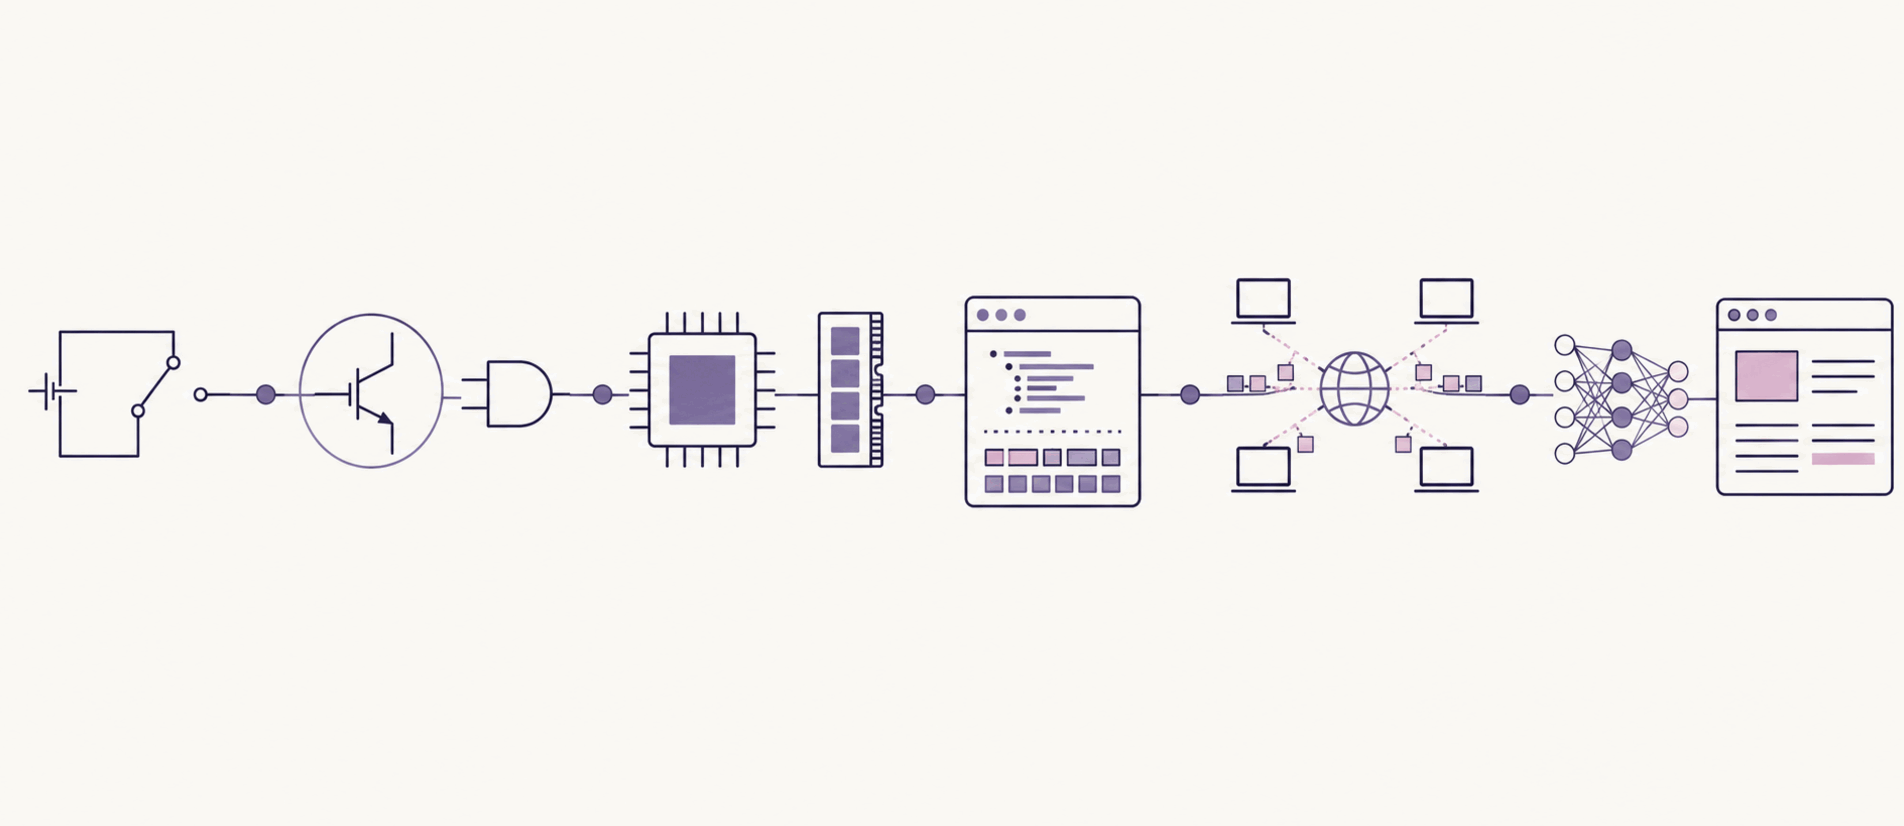
\includegraphics[width=0.95\linewidth]{assets/cover-progression.png}
  \caption{一つの送信を、物理的な信号からアプリケーションの応答までたどる経路}
  \label{fig:learning-progression}
\end{figure}

図\ref{fig:learning-progression}は一方向の階段に見えますが、実際の処理は層を何度も往復します。アプリがOSへ通信を頼めば、CPUがOSの命令を実行します。モデルがメモリから重みを読むたび、キャッシュと回路が働きます。上位の意味は下位の仕組みによって運ばれ、下位で起きた遅延や制限は上位の体験へ戻ってきます。

\section{読者}

主な読者は、アプリケーション開発へ配属される新卒エンジニアです。変数、条件分岐、関数を使った短いプログラムを読んだ経験は想定しますが、電子回路、OS、ネットワーク、機械学習の専門知識は前提にしません。

例にはGoとPythonという二つのプログラミング言語、およびOSへ文字で操作を指示するシェルコマンドを使います。プログラムの書き方の規則である構文そのものより、ある値がどこで生まれ、誰に渡り、いつ消えるかを読み取ります。使用言語が異なっても、同じ役割を持つ仕組みへ置き換えれば物語の筋は変わりません。

\section{読み進め方}

まずは冒頭のリクエストを頭に置き、順番に読み進めてください。本書では、専門用語が初めて現れる場所で太字にし、まず日常語で「何を指すか」を説明します。略語は元の名前を示し、仕組みを説明するために別の専門用語が必要なら、その語を先に説明します。後の章で同じ語が再登場したときは、初出の説明を土台に内部へ一段深く降ります。

用語の意味を読んだら、「今のリクエストのどこで必要になるか」まで確かめてください。図は部品の配置を、コードとコマンドは説明を現実へ結び付ける観測窓を示します。一度説明した語も、しばらく間が空く場所では短く意味を添えます。

節の途中には、厳密さのための数式、仕様上の条件、実装差も登場します。それらは物語から外れた寄り道ではありません。上位の便利な言葉だけでは説明できない瞬間に、どこまで降りれば十分かを知るための手掛かりです。最初は大きな流れをつかみ、二度目に必要な細部へ戻る読み方でも構いません。

章末では、結論を暗記する代わりに、ここまで来たリクエストを自分の言葉でたどり直します。問いや実習へ取り組むときは、結論だけでなく、どの表現を受け取り、どの仕組みが働き、何を次へ渡したかを説明してください。

\takeaway{この本を貫く問いは一つです。送信ボタンを押してから応答が現れるまでに、データはどんな姿へ変わり、誰から誰へ渡されるのでしょうか。}
